\documentclass[a4paper]{jpconf}
\usepackage{graphicx}
\usepackage{url}

\begin{document}
\title{Evolution of the CMS Submission Infrastructure to support heterogeneous resources in the LHC Run 3}

\author{Antonio Pérez-Calero Yzquierdo$^{1,2}$, Edita Kizinevic$^3$, Farrukh Aftab Khan$^4$, Hyunwoo Kim$^4$, Marco Mascheroni$^5$, Maria Acosta Flechas$^4$, Nikos Tsipinakis$^3$ and Saqib Haleem$^6$ on behalf of the CMS Collaboration}
\address{$^1$ Port d'Informaci\'o Cientifica (PIC), Barcelona, Spain}
\address{$^2$ Centro de Investigaciones Energ\'eticas, Medioambientales y Tecnol\'ogicas (CIEMAT), Madrid, Spain}
\address{$^3$ European Organization for Nuclear Research (CERN), Geneva, Switzerland}
\address{$^4$ Fermi National Accelerator Laboratory, Batavia, IL, USA}
\address{$^5$ University of California San Diego, La Jolla, CA, USA}
\address{$^6$ National Centre for Physics, Islamabad, Pakistan}

\ead{aperez@pic.es}

\begin{abstract}
The landscape of computing power available for the CMS experiment is rapidly evolving, from a scenario dominated by x86 processors deployed at WLCG sites towards a more diverse mixture of Grid, HPC, and Cloud facilities, incorporating a higher fraction of non-CPU components such as GPUs. Using these facilities’ heterogeneous resources efficiently to process the vast amounts of data to be collected in the LHC Run 3 and beyond, is key to CMS achieving its scientific goals. The Submission Infrastructure is the main component of the resource acquisition and workload to resource matchmaking systems in CMS Offline Computing. It is therefore firstly mandatory to adapt this infrastructure to be able to request and aggregate heterogeneous resources from our providers and to integrate them into the CMS HTCondor infrastructure. Secondly, it is crucial to optimize the matchmaking of CMS workloads to heterogeneous resources, in order for CMS to succeed in effectively exploiting the enormous amount of computing power that is expected to be available in the form of GPUs. This report presents how this has been technically achieved, as well as a brief description of the already existing pool of GPUs ready for CMS use.

\end{abstract}

\section{The CMS Submission Infrastructure}\label{sec:intro}
The CMS~\cite{cms} Submission Infrastructure (SI) is the main computing resource provisioning system for CMS workflows, including data processing, simulation and analysis. The SI team manages the organization of HTCondor~\cite{htcondor} and GlideinWMS~\cite{gwms} operations that maintain a pool of worldwide distributed compute resources, aggregated from about 70 WLCG~\cite{wlcg} sites, as well as HPC, Cloud, and volunteer providers, for a current total of nearly 400k CPU cores. 

All the allocated resources are managed by a set of federated HTCondor pools, which provide stability and flexibility in the acquisition and utilization of these resources by CMS compute needs. The main component of this infrastructure is the SI Global Pool~\cite{globalpool}\cite{sicomplexity}. 

%The SI group is also responsible for communicating CMS priorities to the development teams of glideinWMS and HTCondor. Discussions about new feature requests and future scale requirements are regularly held at weekly meetings with HTCondor and glideinWMS developers. 
%Operating such an ever growing collection of computing resources that connects different types of resources  (including non-x86 architectures and GPUs) and sources poses significant challenges. Specifically, the SI team is responsible for ensuring the stability of the pool of resources, maximizing data processing throughput, and enforcing task priorities according to the CMS research programme. 
%Overall, the CMS SI team plays a critical role in managing the operations of the CMS distributed pool of compute resources, which is essential for the success of the CMS research programme.

\section{Resource allocation and use in the Global Pool}\label{sec:allocation}
The allocation and utilization of resources in the CMS Global Pool involves a two-stage matchmaking process, as shown in Figure~\ref{fig:pilots}. The first one involves resource allocation to the pool using pilot jobs~\cite{pilots} as requests determined by the GlideinWMS Frontend (FE) and submitted by the pilot $factories$ to Compute Elements (CEs) at WLCG sites. Once these requests have been granted by resource providers, their compute capacity is added to the pool. A subsequent stage then consists of these resource slots, now part of the HTCondor Global Pool, being assigned as dynamically partitioned execution slots for CMS tasks (usually referred to as $payload$ jobs) by the HTCondor $negotiator$. 

\begin{figure}
\begin{center}
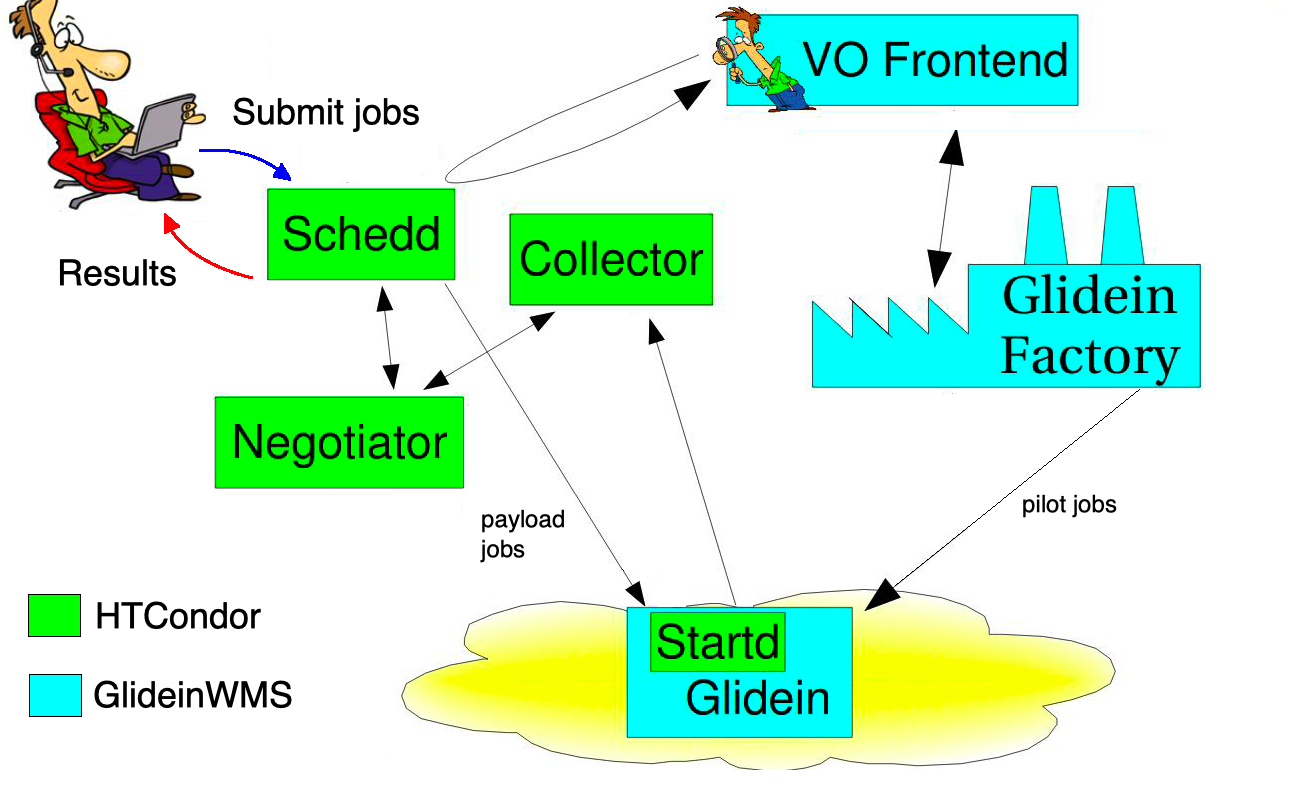
\includegraphics[width=10cm]{figures/glideinwms_pilots.png}
\end{center}
\caption{\label{fig:pilots}GlideinWMS and HTCondor components building a dynamically sized pool of compute resources.}
\end{figure}

\section{Allocation and utilization of heterogeneous resources in the Global Pool}\label{sec:gpu_allocation}
The allocation and use of heterogeneous resources follow the same general logic described in the previous section. However, the SI, along with other elements in the CMS workload management, has been modified in their strategies and scope to make use of these new resource types.

The fact that all GPUs available to CMS at grid sites are so far opportunistic, and not pledged, presents two aspects that separate them from the regular CPU resources employed predominantly up to now. First of all, there is no concept of a regular execution slot, predetermined and agreed upon by the LHC collaborations and the WLCG. Sites have been therefore incorporating GPUs to their infrastructures based on the needs of their local researcher communities, acquisition opportunities, etc. This has resulted in a wide variety of GPU technologies being simultaneously available, diverse in their specifications and performance (more details to this in section~\ref{sec:test}). 

Secondly, being opportunistic, each resource provider may also define their particular allocation policies independently from CMS (e.g available resource types and priority of access to them, maximum number of allocated resources at once, maximum execution time, etc), again contrasting with the uniform policies typical to the system of resource pledges. In this situation, the SI needs to ensure the efficient allocation of resources and their matchmaking to tasks in order to maximize their use by CMS. This requires exploring the optimal level of granularity in the description of the slots, as well as defining new prioritized matchmaking rules for CMS workflows in this emergent resource mix. 

Considering the first matchmaking phase (the acquisition of slots from the grid providers), GPU resource descriptions are encoded statically in the pilot factories. Limited information is available at this point, including basically which sites and CEs can grant CMS access to GPUs, what their associated batch queue names are, etc. Based on this limited information, pilots jobs are submitted in response to the presence of GPU-like workloads in the job scheduler queues. 

However, once a pilot job starts its execution on the remote GPU resources, the \verb|condor_gpu_discovery| tool~\cite{condorgpudiscovery} is employed to retrieve the co-processor properties. In addition, a custom CMS script is used to evaluate the CUDA~\cite{cuda} supported runtime environments. All of this dynamically obtained information is updated in the slot description and can then be used as part of the matchmaking attributes, including:

\begin{verbatim}[CPUs, TotalSlotMemory, GPUs, CUDACapability, CUDAClockMhz, CUDAComputeUnits, 
CUDACoresPerCU, CUDADeviceName, CUDADriverVersion, CUDAECCEnabled, CUDAGlobal
MemoryMB, CUDAMaxSupportedVersion, CMS_CUDA_SUPPORTED_RUNTIMES, CMS_NVIDIA_
DRIVER_VERSION}\end{verbatim}

The description of CMS tasks also requires to be enlarged, starting by identifying those jobs that are suitable for execution using co-processors. A first condition, \verb|RequiresGPU|, defines whether or not the payload job must use a GPU, and therefore should be accounted for in the first matchmaking, when the GlideinWMS FE calculates the resource requests to be submitted onto CEs. A second condition, \verb|RequestGPUs|, determines whether or not jobs can make use of Global Pool GPUs. At the second (HTCondor) matchmaking phase, jobs susceptible of being executed at GPUs can include use specific requirements such as: 
\begin{verbatim} Requirements = CUDACapability >= 3 and CUDARuntime = "11.4"\end{verbatim}

%Finally, the following is used for as matchmaking expression:
%\begin{verbatim}
%Machine.CUDACapability in Job.CUDACapability
%Job.CUDARuntime in Machine.CMS_CUDA_SUPPORTED_RUNTIMES
%Job.GPUs  Machine.GPUs
%\end{verbatim}

%TODO verify all of the above => Antonio: I simplified it in the text to reduce space.

\section{Scale and performance test on GPUs in the CMS Global Pool}\label{sec:test}
To ensure the Global Pool is capable of allocating and providing GPUs to CMS users, the SI team conducted a scale and performance exercise, injecting about 15,000 test jobs targeting any available GPU. The objectives were to match as many GPUs as possible for a period of 24h, and thus conduct a survey how many were available, their location and specifications, as well as assessing their performance on a test computational task. A simple TensorFlow multiple random matrix (10k x 10k, float16) multiplication script was used as the GPU payload. 

A peak allocation of over 150 GPUs in parallel was achieved in the Global Pool (see Figure~\ref{fig:GPUjobs}), with a total of about 230 distinct opportunistic GPUs discovered during the test, with their specifications sumarized in Figure~\ref{fig:GPUdiversity}, located at CERN as well as in several European and US sites. The execution times for the test job was recorded as a function of location and GPU type(shown in Figure~\ref{fig:GPUperformance}), providing valuable insights into the performance of different accelerator types and their suitability for different tasks.

\begin{figure}
\begin{center}
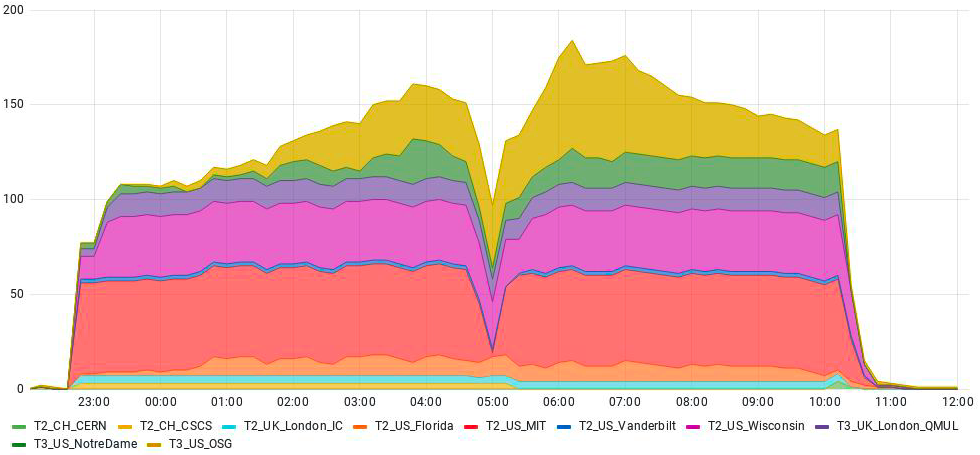
\includegraphics[width=10cm]{figures/GPU_jobs.png}
\end{center}
\caption{\label{fig:GPUjobs}Number of test jobs in simultaneously running on GPUs in the Global Pool, indicating their execution site.}
\end{figure}

\begin{figure}
\begin{center}
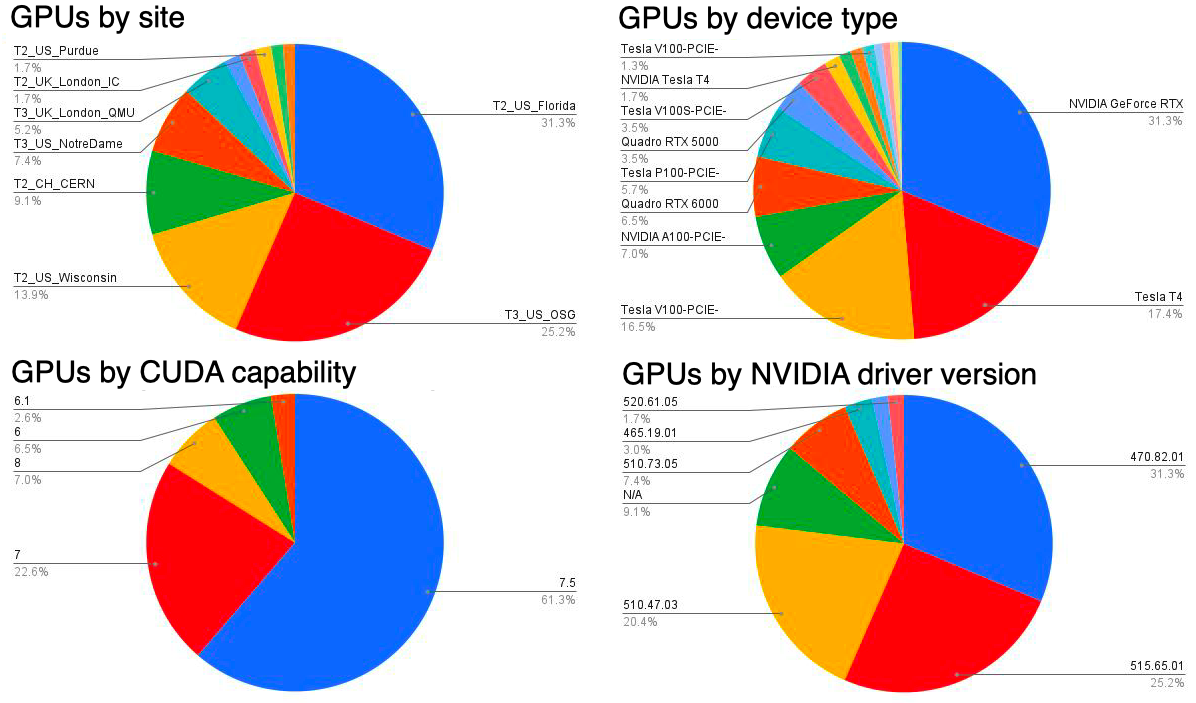
\includegraphics[width=10cm]{figures/GPU_diversity.png}
\end{center}
\caption{\label{fig:GPUdiversity}Diversity of GPUs found during the tests, according to their location at WLCG sites, device type, CUDA capability and NVIDIA driver.}
\end{figure}

\begin{figure}
\begin{center}
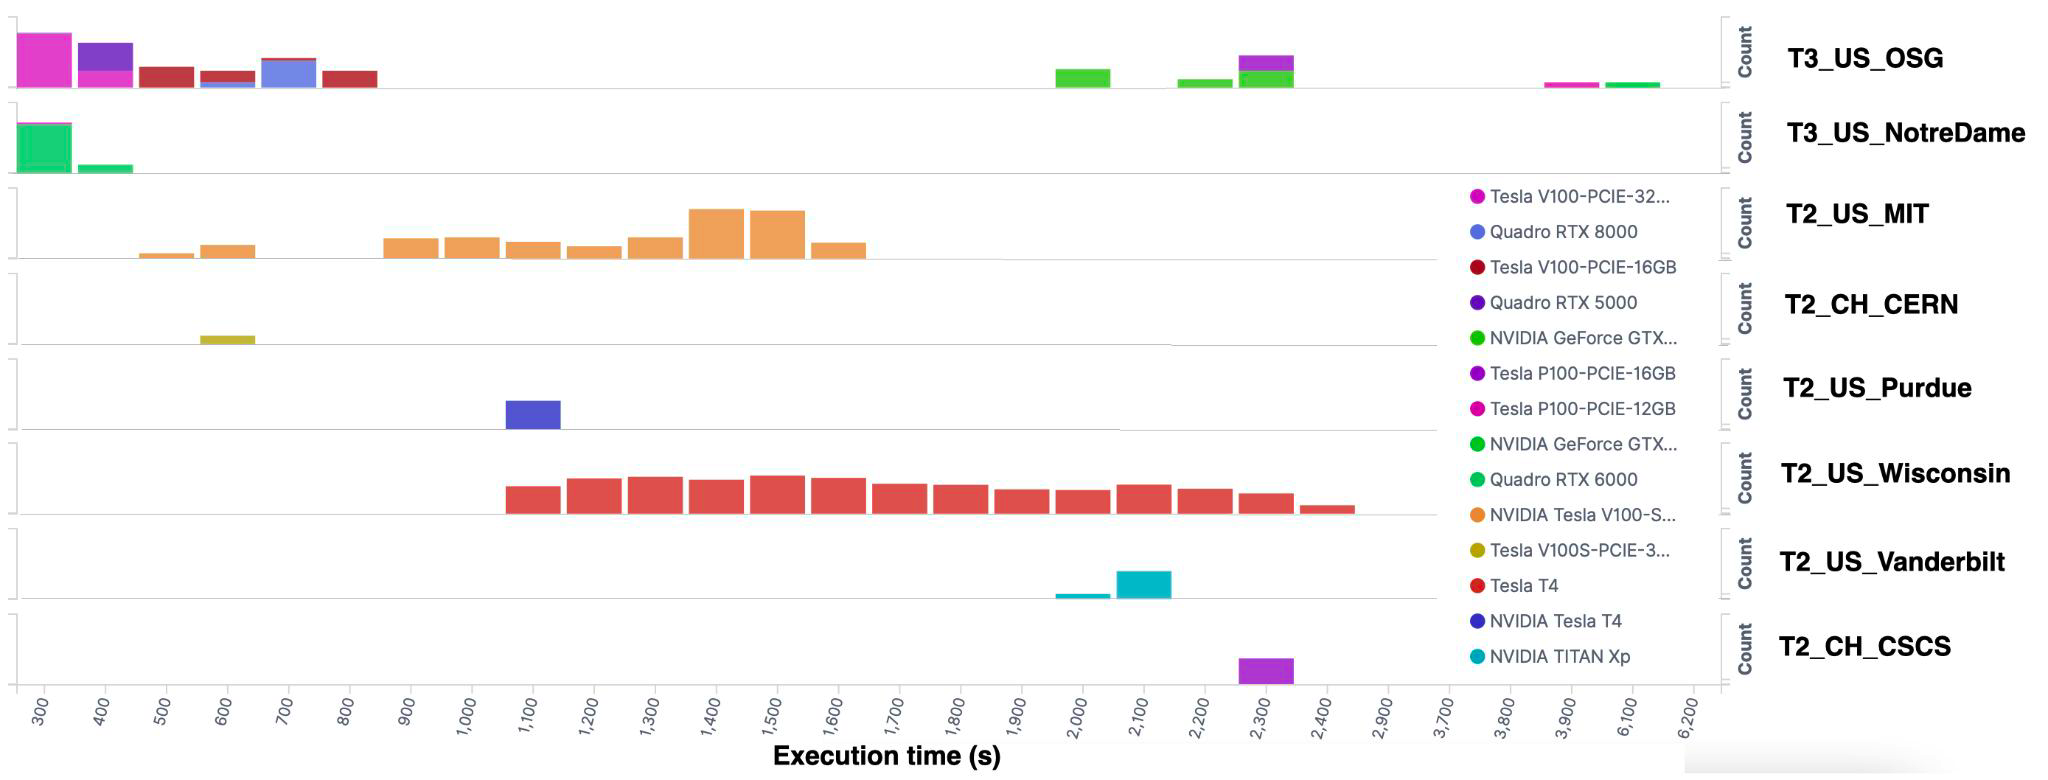
\includegraphics[width=10cm]{figures/GPU_performance.png}
\end{center}
\caption{\label{fig:GPUperformance}Distribution of execution times for the GPU test jobs, as a function of WLCG site and device model.}
\end{figure}

%The SI team has set up a continuous monitoring service to monitor GPU performance to optimize resource allocation to ensure that the CMS Global Pool provides the best possible infrastructure for the reconstruction, simulation, and analysis of CMS data.

\section{Further Challenges in the use of GPUs}\label{sec:challenges}
While the test described provided valuable insights into the allocation and use of GPUs in the CMS Global Pool, CMS faces additional challenges in the use of GPUs originating from the lack of a GPU benchmark adopted by the WLCG. Firstly, this is a requirement for the pledge procedure, as compute needs are assessed by the experiments in terms of a given benchmark, used then by resource providers for their acquisition. Moreover, the lack of a suitable benchmark makes the estimation of predictable workflow execution times (a key parameter for an efficient matchmaking of jobs to slots) extremely difficult in a scenario with high heterogeneity among the available GPUs (as shown in Figure~\ref{fig:GPUperformance}). Lacking a standard benchmark scale widely adopted by the WLCG also prevents sites and experiments from converging on a reliable accounting of the resources provided and used. Lastly, the efficient execution of CMS multi-step jobs~\cite{stepchain} on heterogeneous resources, being only partially compatible with GPUs, remains to be solved.  

%To address this challenge, the SI team uses HTCondor's  \verb|GPUsAverageUsage| as a proxy for GPU resource benchmarking. A cron job uses the NVIDIA driver and tools libraries to query statistics on all of the GPUs and generate a resource usage report. This report provides valuable information on GPU utilization and helps the SI team to identify underutilized or overutilized resources.

%Despite these challenges, the SI team is committed to providing the best possible infrastructure for the reconstruction, simulation, and analysis of CMS data using GPUs. The team continues to explore new solutions to optimize the allocation and use of GPUs in the global pool and to improve the efficiency of job to slot matchmaking. By addressing these challenges, the CMS Global Pool will continue to provide a powerful and reliable computing resource for CMS researchers.

\section{Conclusions and future work}\label{sec:conclusions}
As described in this report, the CMS Submission Infrastructure plays a crucial role in CMS computing operations, managing the acquisition of resources from our providers (WLCG, HPC or Cloud) and workload to resource matchmaking. The integration of heterogeneous resources, such as GPUs, into the SI design, along with a generalization of the matchmaking policies, are requirements to successfully harnessing their potential for CMS use. This note has outlined the methodology to achieve effective scheduling of workflows on GPUs relying on a detailed description of slot properties and task requirements, 

As demonstrated by the exercise described, despite being considered opportunistic resources from WLCG perspective, there is already an existing pool of GPUs available for CMS use. However, the conducted survey also showed that there is no standard description yet for a generic ``GPU slot", thus resulting in unpredictable execution times and potentially reducing the effective use of this type of resources.

The SI team is committed to continue providing a powerful and reliable computing resource for CMS researchers in the form of a Global Pool, now incorporating heterogeneous resources, and to maintaining a regularly updated detailed inventory of available GPUs in order to promote their exploitation by CMS users. To this end, the \verb|condor_ssh_to_job| debugging tool is expected to be a useful addition planned to soon be enabled the CMS SI.

\ack
This work was partially supported by the Spanish Ministry of Science and Innovation under grants PID2019-110942RB-C21, PID2019-110942RB-C22 and PID2020-113807RA-I00, which include FEDER funds from the European Union, and by the US National Science Foundation under Grant No. 2121686
 
\section*{References}
\begin{thebibliography}{9}
\bibitem{cms} CMS Collaboration, The CMS experiment at the CERN LHC, 
JINST 3 (2008) S08004, doi:10.1088/1748-0221/3/08/S08004.
\bibitem{htcondor} The HTCondor Software Suite public web site, \url{https://research.cs.wisc.edu/htcondor/index.html}, accessed March, 2023.
\bibitem{gwms} The Glidein-based Workflow Management System, \url{https://glideinwms.fnal.gov/doc.prd/index.html}, accessed March, 2023.
\bibitem{wlcg} The Worldwide LHC Computing Grid \url{http://wlcg.web.cern.ch}, accessed March, 2023.
\bibitem{globalpool} J. Balcas et al. ``Using the glideinWMS System as a Common Resource Provisioning Layer in CMS'', J. Phys.: Conf. Ser. \textbf{664} 062031 (2015).
\bibitem{sicomplexity} A. Perez-Calero Yzquierdo et al. ``Evolution of the CMS Global Submission Infrastructure for the HL-LHC Era", EPJ Web Conf. 245 (2020) 03016.
\bibitem{pilots} I. Sfiligoi et al. ``The Pilot Way to Grid Resources Using glideinWMS", 2009 WRI World Congress on Computer Science and Information Engineering, Los Angeles, CA, USA, 2009, pp. 428-432, doi: 10.1109/CSIE.2009.950.
\bibitem{condorgpudiscovery} HTCondor gpu discovery tool, \url{https://htcondor.readthedocs.io/en/latest/man-pages/condor_gpu_discovery.html}, accessed March, 2023.
\bibitem{cuda} Compute Unified Device Architecture, CUDA, \url{https://developer.nvidia.com/cuda-zone}, accessed March, 2023.
\bibitem{stepchain} CMS WM team description of single vs multiple step tasks, \url{https://github.com/dmwm/WMCore/wiki/TaskChain-vs-StepChain}, accessed March, 2023.
\bibitem{sshtojob} HTCondor condor\_ssh\_to\_job tool, \url{https://htcondor.readthedocs.io/en/latest/man-pages/condor_ssh_to_job.html}, accessed March, 2023.
\end{thebibliography}

\end{document}
